%% Submissions for peer-review must enable line-numbering
%% using the lineno option in the \documentclass command.
%%
%% Preprints and camera-ready submissions do not need
%% line numbers, and should have this option removed.
%%
%% Please note that the line numbering option requires
%% version 1.1 or newer of the wlpeerj.cls file, and
%% the corresponding author info requires v1.2

\documentclass[fleqn,10pt,lineno]{wlpeerj} % for journal submissions

% ZNK -- Adding headers for pandoc

\setlength{\emergencystretch}{3em}
\providecommand{\tightlist}{
\setlength{\itemsep}{0pt}\setlength{\parskip}{0pt}}
\usepackage{lipsum}
\usepackage[unicode=true]{hyperref}
\usepackage{longtable}


% Pandoc syntax highlighting
% See https://github.com/rstudio/rticles/issues/182
\usepackage{color}
\usepackage{fancyvrb}
\newcommand{\VerbBar}{|}
\newcommand{\VERB}{\Verb[commandchars=\\\{\}]}
\DefineVerbatimEnvironment{Highlighting}{Verbatim}{commandchars=\\\{\}}
% Add ',fontsize=\small' for more characters per line
\usepackage{framed}
\definecolor{shadecolor}{RGB}{248,248,248}
\newenvironment{Shaded}{\begin{snugshade}}{\end{snugshade}}
\newcommand{\AlertTok}[1]{\textcolor[rgb]{0.94,0.16,0.16}{#1}}
\newcommand{\AnnotationTok}[1]{\textcolor[rgb]{0.56,0.35,0.01}{\textbf{\textit{#1}}}}
\newcommand{\AttributeTok}[1]{\textcolor[rgb]{0.77,0.63,0.00}{#1}}
\newcommand{\BaseNTok}[1]{\textcolor[rgb]{0.00,0.00,0.81}{#1}}
\newcommand{\BuiltInTok}[1]{#1}
\newcommand{\CharTok}[1]{\textcolor[rgb]{0.31,0.60,0.02}{#1}}
\newcommand{\CommentTok}[1]{\textcolor[rgb]{0.56,0.35,0.01}{\textit{#1}}}
\newcommand{\CommentVarTok}[1]{\textcolor[rgb]{0.56,0.35,0.01}{\textbf{\textit{#1}}}}
\newcommand{\ConstantTok}[1]{\textcolor[rgb]{0.00,0.00,0.00}{#1}}
\newcommand{\ControlFlowTok}[1]{\textcolor[rgb]{0.13,0.29,0.53}{\textbf{#1}}}
\newcommand{\DataTypeTok}[1]{\textcolor[rgb]{0.13,0.29,0.53}{#1}}
\newcommand{\DecValTok}[1]{\textcolor[rgb]{0.00,0.00,0.81}{#1}}
\newcommand{\DocumentationTok}[1]{\textcolor[rgb]{0.56,0.35,0.01}{\textbf{\textit{#1}}}}
\newcommand{\ErrorTok}[1]{\textcolor[rgb]{0.64,0.00,0.00}{\textbf{#1}}}
\newcommand{\ExtensionTok}[1]{#1}
\newcommand{\FloatTok}[1]{\textcolor[rgb]{0.00,0.00,0.81}{#1}}
\newcommand{\FunctionTok}[1]{\textcolor[rgb]{0.00,0.00,0.00}{#1}}
\newcommand{\ImportTok}[1]{#1}
\newcommand{\InformationTok}[1]{\textcolor[rgb]{0.56,0.35,0.01}{\textbf{\textit{#1}}}}
\newcommand{\KeywordTok}[1]{\textcolor[rgb]{0.13,0.29,0.53}{\textbf{#1}}}
\newcommand{\NormalTok}[1]{#1}
\newcommand{\OperatorTok}[1]{\textcolor[rgb]{0.81,0.36,0.00}{\textbf{#1}}}
\newcommand{\OtherTok}[1]{\textcolor[rgb]{0.56,0.35,0.01}{#1}}
\newcommand{\PreprocessorTok}[1]{\textcolor[rgb]{0.56,0.35,0.01}{\textit{#1}}}
\newcommand{\RegionMarkerTok}[1]{#1}
\newcommand{\SpecialCharTok}[1]{\textcolor[rgb]{0.00,0.00,0.00}{#1}}
\newcommand{\SpecialStringTok}[1]{\textcolor[rgb]{0.31,0.60,0.02}{#1}}
\newcommand{\StringTok}[1]{\textcolor[rgb]{0.31,0.60,0.02}{#1}}
\newcommand{\VariableTok}[1]{\textcolor[rgb]{0.00,0.00,0.00}{#1}}
\newcommand{\VerbatimStringTok}[1]{\textcolor[rgb]{0.31,0.60,0.02}{#1}}
\newcommand{\WarningTok}[1]{\textcolor[rgb]{0.56,0.35,0.01}{\textbf{\textit{#1}}}}

% Pandoc Header

\title{Response and adverse events to chemotherapy: A mock study}

\author[RStudio]{Alison Hill, Ph.D.}

\author[University of Michigan]{Peter Higgins, MD, Ph.D.}




%
% \author[1]{First Author}
% \author[2]{Second Author}
% \affil[1]{Address of first author}
% \affil[2]{Address of second author}
% \corrauthor[1]{First Author}{f.author@email.com}

% 

\begin{abstract}

% Dummy abstract text. Dummy abstract text. Dummy abstract text. Dummy abstract text. Dummy abstract text. Dummy abstract text. Dummy abstract text. Dummy abstract text. Dummy abstract text. Dummy abstract text. Dummy abstract text.
\end{abstract}

\begin{document}

\flushbottom
\maketitle
\thispagestyle{empty}

\hypertarget{basic-sanity-checkingeda-here}{%
\section{Basic sanity checking/EDA here}\label{basic-sanity-checkingeda-here}}

\begin{Shaded}
\begin{Highlighting}[]
\KeywordTok{glimpse}\NormalTok{(mockdata)}
\end{Highlighting}
\end{Shaded}

\begin{verbatim}
## Observations: 1,499
## Variables: 25
## $ case        <dbl> 110754, 99706, 105271, 105001, 112263, 86205, 9950...
## $ age         <dbl> 67, 74, 50, 71, 69, 56, 50, 57, 51, 63, 61, 59, 61...
## $ arm         <chr> "F: FOLFOX", "A: IFL", "A: IFL", "G: IROX", "F: FO...
## $ sex         <chr> "Male", "Female", "Female", "Female", "Female", "M...
## $ race        <chr> "Caucasian", "Caucasian", "Caucasian", "Caucasian"...
## $ fu_time     <dbl> 922, 270, 175, 128, 233, 120, 369, 421, 387, 363, ...
## $ fu_stat     <dbl> 2, 2, 2, 2, 2, 2, 2, 2, 2, 2, 2, 2, 2, 2, 1, 2, 2,...
## $ ps          <dbl> 0, 1, 1, 1, 0, 0, 0, 0, 1, 1, 1, 0, 1, 1, 0, 0, 1,...
## $ hgb         <dbl> 11.5, 10.7, 11.1, 12.6, 13.0, 10.2, 13.3, 12.1, 13...
## $ bmi         <dbl> 25.09861, 19.49786, NA, 29.42922, 26.35352, 19.036...
## $ alk_phos    <dbl> 160, 290, 700, 771, 350, 569, 162, 152, 231, 492, ...
## $ ast         <dbl> 35, 52, 100, 68, 35, 27, 16, 12, 25, 18, 45, 16, 5...
## $ mdquality_s <dbl> NA, 1, 1, 1, NA, 1, 1, 1, 1, 1, NA, NA, 1, 0, 1, 1...
## $ age_ord     <chr> "60-69", "70-79", "40-49", "70-79", "60-69", "50-5...
## $ ethnicity   <chr> "White (not Hispanic)", "White (not Hispanic)", "W...
## $ name        <chr> "Daniel Robinson", "Delaney Quinby", "Lauren Ginn"...
## $ first_name  <chr> "Daniel", "Delaney", "Lauren", "Julia", "Iffat", "...
## $ last_name   <chr> "Robinson", "Quinby", "Ginn", "Carney", "al-Sahli"...
## $ low_wbc     <dbl> 0, 0, 0, 0, 0, 0, 1, 1, 0, 0, 0, 0, 0, 0, 0, 0, 0,...
## $ neuropathy  <dbl> 0, 0, 0, 0, 0, 0, 1, 1, 0, 0, 0, 0, 0, 0, 0, 0, 0,...
## $ diarrhea    <dbl> 0, 0, 0, 0, 0, 0, 1, 1, 0, 0, 0, 0, 0, 0, 0, 0, 0,...
## $ vomiting    <dbl> 0, 0, 0, 0, 0, 0, 1, 1, 0, 0, 0, 0, 0, 0, 0, 0, 0,...
## $ blood_clot  <dbl> 0, 0, 0, 0, 0, 0, 0, 0, 0, 0, 0, 0, 0, 0, 0, 0, 0,...
## $ site        <chr> "Portland", "Portland", "Portland", "Portland", "P...
## $ country     <chr> "USA", "USA", "USA", "USA", "USA", "USA", "USA", "...
\end{verbatim}

\begin{Shaded}
\begin{Highlighting}[]
\CommentTok{# skim(mockdata)}

\NormalTok{mockdata }\OperatorTok\StringTok{ }
\StringTok{  }\KeywordTok{group_by}\NormalTok{(arm) }\OperatorTok\StringTok{ }
\StringTok{  }\KeywordTok{skim}\NormalTok{()}
\end{Highlighting}
\end{Shaded}

\begin{verbatim}
## Skim summary statistics
##  n obs: 1499 
##  n variables: 25 
##  group variables: arm 
## 
## -- Variable type:character ------------------------------------------------------------------------------
##        arm   variable missing complete   n min max empty n_unique
##     A: IFL    age_ord       0      428 428   5   5     0        7
##     A: IFL    country       0      428 428   3   5     0        2
##     A: IFL  ethnicity       0      428 428   8  33     0        6
##     A: IFL first_name       0      428 428   2  11     0      279
##     A: IFL  last_name       0      428 428   3  16     0      398
##     A: IFL       name       0      428 428   8  27     0      428
##     A: IFL       race       0      428 428   5  16     0        7
##     A: IFL        sex       0      428 428   4   6     0        2
##     A: IFL       site       0      428 428   6  11     0       13
##  F: FOLFOX    age_ord       0      691 691   5   5     0        8
##  F: FOLFOX    country       0      691 691   3  10     0        5
##  F: FOLFOX  ethnicity       0      691 691   8  33     0        6
##  F: FOLFOX first_name       0      691 691   2  11     0      397
##  F: FOLFOX  last_name       0      691 691   2  16     0      617
##  F: FOLFOX       name       0      691 691   8  27     0      691
##  F: FOLFOX       race       0      691 691   5  16     0        7
##  F: FOLFOX        sex       0      691 691   4   6     0        2
##  F: FOLFOX       site       0      691 691   6  14     0       18
##    G: IROX    age_ord       0      380 380   5   5     0        7
##    G: IROX    country       0      380 380   3   3     0        1
##    G: IROX  ethnicity       0      380 380   8  33     0        6
##    G: IROX first_name       0      380 380   2  11     0      262
##    G: IROX  last_name       0      380 380   3  16     0      357
##    G: IROX       name       0      380 380   9  23     0      380
##    G: IROX       race       0      380 380   5  16     0        7
##    G: IROX        sex       0      380 380   4   6     0        2
##    G: IROX       site       0      380 380   6  11     0       12
## 
## -- Variable type:numeric --------------------------------------------------------------------------------
##        arm    variable missing complete   n      mean      sd       p0
##     A: IFL         age       0      428 428    59.67    11.36    27   
##     A: IFL    alk_phos      69      359 428   175.58   128.61    11   
##     A: IFL         ast      69      359 428    37.29    28.04    10   
##     A: IFL  blood_clot       0      428 428     0.063    0.24     0   
##     A: IFL         bmi       9      419 428    27.29     5.55    14.05
##     A: IFL        case       0      428 428 95252.21  8200.84 76170   
##     A: IFL    diarrhea       0      428 428     0.18     0.39     0   
##     A: IFL     fu_stat       0      428 428     1.96     0.2      1   
##     A: IFL     fu_time       0      428 428   553.58   419.61     9   
##     A: IFL         hgb      69      359 428    12.28     1.69     9.06
##     A: IFL     low_wbc       0      428 428     0.16     0.37     0   
##     A: IFL mdquality_s      55      373 428     0.89     0.31     0   
##     A: IFL  neuropathy       0      428 428     0.16     0.37     0   
##     A: IFL          ps      69      359 428     0.53     0.6      0   
##     A: IFL    vomiting       0      428 428     0.18     0.39     0   
##  F: FOLFOX         age       0      691 691    60.3     11.63    19   
##  F: FOLFOX    alk_phos     141      550 691   161.98   121.98    10   
##  F: FOLFOX         ast     141      550 691    35.2     26.66     7   
##  F: FOLFOX  blood_clot       0      691 691     0.046    0.21     0   
##  F: FOLFOX         bmi      20      671 691    27.21     5.17    16.65
##  F: FOLFOX        case       0      691 691 1e+05     9617.76 78845   
##  F: FOLFOX    diarrhea       0      691 691     0.29     0.45     0   
##  F: FOLFOX     fu_stat       0      691 691     1.86     0.35     1   
##  F: FOLFOX     fu_time       0      691 691   731.25   487.74     0   
##  F: FOLFOX         hgb     141      550 691    12.38     1.76     9   
##  F: FOLFOX     low_wbc       0      691 691     0.26     0.44     0   
##  F: FOLFOX mdquality_s     156      535 691     0.9      0.3      0   
##  F: FOLFOX  neuropathy       0      691 691     0.21     0.41     0   
##  F: FOLFOX          ps     141      550 691     0.55     0.59     0   
##  F: FOLFOX    vomiting       0      691 691     0.25     0.43     0   
##    G: IROX         age       0      380 380    59.76    11.5     26   
##    G: IROX    alk_phos      56      324 380   173.51   138.56     7   
##    G: IROX         ast      56      324 380    35.67    25.81     5   
##    G: IROX  blood_clot       0      380 380     0.039    0.19     0   
##    G: IROX         bmi       4      376 380    27.11     5.75    15.43
##    G: IROX        case       0      380 380 94869.23  6960.2  78841   
##    G: IROX    diarrhea       0      380 380     0.092    0.29     0   
##    G: IROX     fu_stat       0      380 380     1.93     0.25     1   
##    G: IROX     fu_time       0      380 380   607.24   435.51    17   
##    G: IROX         hgb      56      324 380    12.37     1.68     9   
##    G: IROX     low_wbc       0      380 380     0.068    0.25     0   
##    G: IROX mdquality_s      41      339 380     0.91     0.29     0   
##    G: IROX  neuropathy       0      380 380     0.068    0.25     0   
##    G: IROX          ps      56      324 380     0.54     0.61     0   
##    G: IROX    vomiting       0      380 380     0.092    0.29     0   
##       p25       p50       p75      p100     hist
##     53        61        68        88    ▁▂▃▆▇▆▃▁
##     89       133       217       858    ▇▆▂▁▁▁▁▁
##     21        29        42       205    ▇▃▁▁▁▁▁▁
##      0         0         0         1    ▇▁▁▁▁▁▁▁
##     23.57     26.23     30.59     53.01 ▁▅▇▅▂▁▁▁
##  90563     93317     1e+05    108884    ▂▁▂▇▆▁▃▆
##      0         0         0         1    ▇▁▁▁▁▁▁▂
##      2         2         2         2    ▁▁▁▁▁▁▁▇
##    255.5     446.5     724.25   2170    ▇▇▅▂▂▁▁▁
##     11        12.1      13.45     17.3  ▃▇▇▇▆▃▁▁
##      0         0         0         1    ▇▁▁▁▁▁▁▂
##      1         1         1         1    ▁▁▁▁▁▁▁▇
##      0         0         0         1    ▇▁▁▁▁▁▁▂
##      0         0         1         2    ▇▁▁▆▁▁▁▁
##      0         0         0         1    ▇▁▁▁▁▁▁▂
##     52        61        69        88    ▁▁▂▆▇▇▅▁
##     85       116       194.75   1014    ▇▃▁▁▁▁▁▁
##     19        25.5      40       174    ▇▃▁▁▁▁▁▁
##      0         0         0         1    ▇▁▁▁▁▁▁▁
##     23.75     26.52     30.12     49.13 ▂▆▇▅▂▁▁▁
##  92512.5  105126    111018.5  112488    ▁▁▂▃▁▂▂▇
##      0         0         1         1    ▇▁▁▁▁▁▁▃
##      2         2         2         2    ▂▁▁▁▁▁▁▇
##    345       601      1046      2472    ▅▇▅▃▃▁▁▁
##     11.1      12.2      13.6      18.2  ▃▆▇▆▅▂▁▁
##      0         0         1         1    ▇▁▁▁▁▁▁▃
##      1         1         1         1    ▁▁▁▁▁▁▁▇
##      0         0         0         1    ▇▁▁▁▁▁▁▂
##      0         0         1         2    ▇▁▁▇▁▁▁▁
##      0         0         0         1    ▇▁▁▁▁▁▁▂
##     52        61        68        85    ▁▂▂▅▆▇▅▁
##     87.75    122       210.25    982    ▇▅▂▁▁▁▁▁
##     20        27        41       176    ▇▆▂▁▁▁▁▁
##      0         0         0         1    ▇▁▁▁▁▁▁▁
##     23.17     25.98     29.61     60.24 ▂▇▅▂▁▁▁▁
##  90638.75  93126     1e+05    107746    ▁▁▂▇▃▁▃▃
##      0         0         0         1    ▇▁▁▁▁▁▁▁
##      2         2         2         2    ▁▁▁▁▁▁▁▇
##    306.5     515.5     807      2118    ▆▇▆▃▁▁▁▁
##     11.17     12.4      13.62     17    ▃▅▆▇▇▃▂▁
##      0         0         0         1    ▇▁▁▁▁▁▁▁
##      1         1         1         1    ▁▁▁▁▁▁▁▇
##      0         0         0         1    ▇▁▁▁▁▁▁▁
##      0         0         1         2    ▇▁▁▆▁▁▁▁
##      0         0         0         1    ▇▁▁▁▁▁▁▁
\end{verbatim}

\hypertarget{make-table-one-here}{%
\section{Make table one here}\label{make-table-one-here}}

Let's make a basic Table 1 grouped by arm with details on sex and age in each group.

\begin{Shaded}
\begin{Highlighting}[]
\CommentTok{#summary by groups}
\NormalTok{tab1 <-}\StringTok{ }\KeywordTok{tableby}\NormalTok{(arm }\OperatorTok{~}\StringTok{ }\NormalTok{sex }\OperatorTok{+}\StringTok{ }\NormalTok{age, }\DataTypeTok{data =}\NormalTok{ mockdata)}
\KeywordTok{summary}\NormalTok{(tab1, }\DataTypeTok{text=}\OtherTok{TRUE}\NormalTok{)}
\end{Highlighting}
\end{Shaded}

\begin{longtable}[]{@{}lccccr@{}}
\toprule
& A: IFL (N=428) & F: FOLFOX (N=691) & G: IROX (N=380) & Total (N=1499) & p value\tabularnewline
\midrule
\endhead
sex & & & & & 0.190\tabularnewline
- Female & 151 (35.3\%) & 280 (40.5\%) & 152 (40.0\%) & 583 (38.9\%) &\tabularnewline
- Male & 277 (64.7\%) & 411 (59.5\%) & 228 (60.0\%) & 916 (61.1\%) &\tabularnewline
age & & & & & 0.614\tabularnewline
- Mean (SD) & 59.673 (11.365) & 60.301 (11.632) & 59.763 (11.499) & 59.985 (11.519) &\tabularnewline
- Range & 27.000 - 88.000 & 19.000 - 88.000 & 26.000 - 85.000 & 19.000 - 88.000 &\tabularnewline
\bottomrule
\end{longtable}

Let's make a Table 1 - but ungrouped, with stats on BMI, sex, Age in each group.

\begin{Shaded}
\begin{Highlighting}[]
\CommentTok{#summary without groups}
\NormalTok{tab.noby <-}\StringTok{ }\KeywordTok{tableby}\NormalTok{(}\OperatorTok{~}\StringTok{ }\NormalTok{bmi }\OperatorTok{+}\StringTok{ }\NormalTok{sex }\OperatorTok{+}\StringTok{ }\NormalTok{age, }\DataTypeTok{data =}\NormalTok{ mockdata)}
\KeywordTok{summary}\NormalTok{(tab.noby)}
\end{Highlighting}
\end{Shaded}

\begin{longtable}[]{@{}lc@{}}
\toprule
& Overall (N=1499)\tabularnewline
\midrule
\endhead
\textbf{bmi} &\tabularnewline
~~~N-Miss & 33\tabularnewline
~~~Mean (SD) & 27.206 (5.432)\tabularnewline
~~~Range & 14.053 - 60.243\tabularnewline
\textbf{sex} &\tabularnewline
~~~Female & 583 (38.9\%)\tabularnewline
~~~Male & 916 (61.1\%)\tabularnewline
\textbf{age} &\tabularnewline
~~~Mean (SD) & 59.985 (11.519)\tabularnewline
~~~Range & 19.000 - 88.000\tabularnewline
\bottomrule
\end{longtable}

Let's make a Table 1 but now control \# of digits

\begin{Shaded}
\begin{Highlighting}[]
\KeywordTok{summary}\NormalTok{(}\KeywordTok{tableby}\NormalTok{(arm }\OperatorTok{~}\StringTok{ }\NormalTok{sex }\OperatorTok{+}\StringTok{ }\NormalTok{fu_time, }\DataTypeTok{data =}\NormalTok{ mockdata), }
        \DataTypeTok{digits =} \DecValTok{4}\NormalTok{, }\DataTypeTok{digits.p =} \DecValTok{2}\NormalTok{, }\DataTypeTok{digits.pct =} \DecValTok{1}\NormalTok{)}
\end{Highlighting}
\end{Shaded}

\begin{longtable}[]{@{}lccccr@{}}
\toprule
\begin{minipage}[b]{0.19\columnwidth}\raggedright
\strut
\end{minipage} & \begin{minipage}[b]{0.15\columnwidth}\centering
A: IFL (N=428)\strut
\end{minipage} & \begin{minipage}[b]{0.15\columnwidth}\centering
F: FOLFOX (N=691)\strut
\end{minipage} & \begin{minipage}[b]{0.15\columnwidth}\centering
G: IROX (N=380)\strut
\end{minipage} & \begin{minipage}[b]{0.15\columnwidth}\centering
Total (N=1499)\strut
\end{minipage} & \begin{minipage}[b]{0.06\columnwidth}\raggedleft
p value\strut
\end{minipage}\tabularnewline
\midrule
\endhead
\begin{minipage}[t]{0.19\columnwidth}\raggedright
\textbf{sex}\strut
\end{minipage} & \begin{minipage}[t]{0.15\columnwidth}\centering
\strut
\end{minipage} & \begin{minipage}[t]{0.15\columnwidth}\centering
\strut
\end{minipage} & \begin{minipage}[t]{0.15\columnwidth}\centering
\strut
\end{minipage} & \begin{minipage}[t]{0.15\columnwidth}\centering
\strut
\end{minipage} & \begin{minipage}[t]{0.06\columnwidth}\raggedleft
0.19\strut
\end{minipage}\tabularnewline
\begin{minipage}[t]{0.19\columnwidth}\raggedright
~~~Female\strut
\end{minipage} & \begin{minipage}[t]{0.15\columnwidth}\centering
151 (35.3\%)\strut
\end{minipage} & \begin{minipage}[t]{0.15\columnwidth}\centering
280 (40.5\%)\strut
\end{minipage} & \begin{minipage}[t]{0.15\columnwidth}\centering
152 (40.0\%)\strut
\end{minipage} & \begin{minipage}[t]{0.15\columnwidth}\centering
583 (38.9\%)\strut
\end{minipage} & \begin{minipage}[t]{0.06\columnwidth}\raggedleft
\strut
\end{minipage}\tabularnewline
\begin{minipage}[t]{0.19\columnwidth}\raggedright
~~~Male\strut
\end{minipage} & \begin{minipage}[t]{0.15\columnwidth}\centering
277 (64.7\%)\strut
\end{minipage} & \begin{minipage}[t]{0.15\columnwidth}\centering
411 (59.5\%)\strut
\end{minipage} & \begin{minipage}[t]{0.15\columnwidth}\centering
228 (60.0\%)\strut
\end{minipage} & \begin{minipage}[t]{0.15\columnwidth}\centering
916 (61.1\%)\strut
\end{minipage} & \begin{minipage}[t]{0.06\columnwidth}\raggedleft
\strut
\end{minipage}\tabularnewline
\begin{minipage}[t]{0.19\columnwidth}\raggedright
\textbf{fu\_time}\strut
\end{minipage} & \begin{minipage}[t]{0.15\columnwidth}\centering
\strut
\end{minipage} & \begin{minipage}[t]{0.15\columnwidth}\centering
\strut
\end{minipage} & \begin{minipage}[t]{0.15\columnwidth}\centering
\strut
\end{minipage} & \begin{minipage}[t]{0.15\columnwidth}\centering
\strut
\end{minipage} & \begin{minipage}[t]{0.06\columnwidth}\raggedleft
\textless{} 0.01\strut
\end{minipage}\tabularnewline
\begin{minipage}[t]{0.19\columnwidth}\raggedright
~~~Mean (SD)\strut
\end{minipage} & \begin{minipage}[t]{0.15\columnwidth}\centering
553.5841 (419.6065)\strut
\end{minipage} & \begin{minipage}[t]{0.15\columnwidth}\centering
731.2460 (487.7443)\strut
\end{minipage} & \begin{minipage}[t]{0.15\columnwidth}\centering
607.2421 (435.5092)\strut
\end{minipage} & \begin{minipage}[t]{0.15\columnwidth}\centering
649.0841 (462.5109)\strut
\end{minipage} & \begin{minipage}[t]{0.06\columnwidth}\raggedleft
\strut
\end{minipage}\tabularnewline
\begin{minipage}[t]{0.19\columnwidth}\raggedright
~~~Range\strut
\end{minipage} & \begin{minipage}[t]{0.15\columnwidth}\centering
9.0000 - 2170.0000\strut
\end{minipage} & \begin{minipage}[t]{0.15\columnwidth}\centering
0.0000 - 2472.0000\strut
\end{minipage} & \begin{minipage}[t]{0.15\columnwidth}\centering
17.0000 - 2118.0000\strut
\end{minipage} & \begin{minipage}[t]{0.15\columnwidth}\centering
0.0000 - 2472.0000\strut
\end{minipage} & \begin{minipage}[t]{0.06\columnwidth}\raggedleft
\strut
\end{minipage}\tabularnewline
\bottomrule
\end{longtable}

\hypertarget{run-some-stats-and-make-a-table-here}{%
\section{Run some stats and make a table here}\label{run-some-stats-and-make-a-table-here}}

Arm x fu\_stat chi square table (1 = lived, 2 = died)

\begin{Shaded}
\begin{Highlighting}[]
\NormalTok{mockdata }\OperatorTok\StringTok{ }
\StringTok{  }\KeywordTok{tabyl}\NormalTok{(arm, fu_stat) }\OperatorTok\StringTok{ }
\StringTok{  }\KeywordTok{adorn_totals}\NormalTok{(}\StringTok{"row"}\NormalTok{) }\OperatorTok\StringTok{ }\CommentTok{# can also do "col", or c("row", "col")}
\StringTok{  }\KeywordTok{adorn_percentages}\NormalTok{() }\OperatorTok\StringTok{ }
\StringTok{  }\KeywordTok{adorn_pct_formatting}\NormalTok{() }\OperatorTok\StringTok{ }
\StringTok{  }\KeywordTok{adorn_ns}\NormalTok{() }\OperatorTok\StringTok{ }
\StringTok{  }\NormalTok{knitr}\OperatorTok{::}\KeywordTok{kable}\NormalTok{()}
\end{Highlighting}
\end{Shaded}

\begin{tabular}{l|l|l}
\hline
arm & 1 & 2\\
\hline
A: IFL & 4.2\%  (18) & 95.8\%  (410)\\
\hline
F: FOLFOX & 14.3\%  (99) & 85.7\%  (592)\\
\hline
G: IROX & 6.8\%  (26) & 93.2\%  (354)\\
\hline
Total & 9.5\% (143) & 90.5\% (1356)\\
\hline
\end{tabular}

\begin{Shaded}
\begin{Highlighting}[]
\NormalTok{mockdata }\OperatorTok\StringTok{ }
\StringTok{  }\KeywordTok{specify}\NormalTok{(fu_stat }\OperatorTok{~}\StringTok{ }\NormalTok{arm) }\OperatorTok\StringTok{ }\CommentTok{# alt: response = fu_stat, explanatory = arm}
\StringTok{  }\KeywordTok{calculate}\NormalTok{(}\DataTypeTok{stat =} \StringTok{"Chisq"}\NormalTok{)}
\end{Highlighting}
\end{Shaded}

\begin{Shaded}
\begin{Highlighting}[]
\NormalTok{mockdata }\OperatorTok\StringTok{ }
\StringTok{  }\KeywordTok{specify}\NormalTok{(}\DataTypeTok{formula =}\NormalTok{ fu_stat }\OperatorTok{~}\StringTok{ }\NormalTok{arm, }\DataTypeTok{success =} \StringTok{"1"}\NormalTok{) }\OperatorTok\StringTok{ }
\StringTok{  }\KeywordTok{hypothesize}\NormalTok{(}\DataTypeTok{null =} \StringTok{"independence"}\NormalTok{) }\OperatorTok\StringTok{ }
\StringTok{  }\KeywordTok{generate}\NormalTok{(}\DataTypeTok{reps =} \DecValTok{1000}\NormalTok{, }\DataTypeTok{type =} \StringTok{"permute"}\NormalTok{) }\OperatorTok\StringTok{ }
\StringTok{  }\KeywordTok{calculate}\NormalTok{(}\DataTypeTok{stat =} \StringTok{"diff in props"}\NormalTok{, }\DataTypeTok{order =} \KeywordTok{c}\NormalTok{(}\StringTok{"1"}\NormalTok{, }\StringTok{"2"}\NormalTok{))}
\end{Highlighting}
\end{Shaded}

make bar/lollipop chart of proportions here (\% survived)

Start with a barplot
for percent survival
tag it as panel A for a multipanel plot

\begin{Shaded}
\begin{Highlighting}[]
\NormalTok{mockdata }\OperatorTok\StringTok{ }
\StringTok{  }\KeywordTok{group_by}\NormalTok{(arm) }\OperatorTok\StringTok{ }
\StringTok{  }\KeywordTok{summarize}\NormalTok{(}\DataTypeTok{surv =} \KeywordTok{length}\NormalTok{(}\KeywordTok{which}\NormalTok{(fu_stat}\OperatorTok{==}\DecValTok{1}\NormalTok{)),}
         \DataTypeTok{died =} \KeywordTok{length}\NormalTok{(}\KeywordTok{which}\NormalTok{(fu_stat}\OperatorTok{==}\DecValTok{2}\NormalTok{)),}
         \DataTypeTok{pct_surv =}\NormalTok{ surv}\OperatorTok{*}\DecValTok{100}\OperatorTok{/}\NormalTok{(died}\OperatorTok{+}\NormalTok{surv)) }\OperatorTok\StringTok{ }
\StringTok{  }\KeywordTok{select}\NormalTok{(arm, surv, died, pct_surv) }\OperatorTok\StringTok{ }
\StringTok{  }\KeywordTok{ggplot}\NormalTok{() }\OperatorTok{+}
\StringTok{  }\KeywordTok{aes}\NormalTok{(}\DataTypeTok{x=}\NormalTok{arm, }\DataTypeTok{y =}\NormalTok{ pct_surv, }\DataTypeTok{fill=}\NormalTok{arm) }\OperatorTok{+}
\StringTok{  }\KeywordTok{geom_col}\NormalTok{(}\DataTypeTok{colour =} \StringTok{"gray"}\NormalTok{) }\OperatorTok{+}
\StringTok{  }\KeywordTok{labs}\NormalTok{(}\DataTypeTok{y=} \StringTok{"Percent Survived"}\NormalTok{, }\DataTypeTok{x=} \StringTok{"Study Arm"}\NormalTok{, }\DataTypeTok{tag =}\StringTok{"A"}\NormalTok{) }\OperatorTok{+}
\StringTok{  }\KeywordTok{scale_fill_scico_d}\NormalTok{(}\DataTypeTok{palette =} \StringTok{'nuuk'}\NormalTok{)  ->}
\NormalTok{p1}

\NormalTok{p1}
\end{Highlighting}
\end{Shaded}

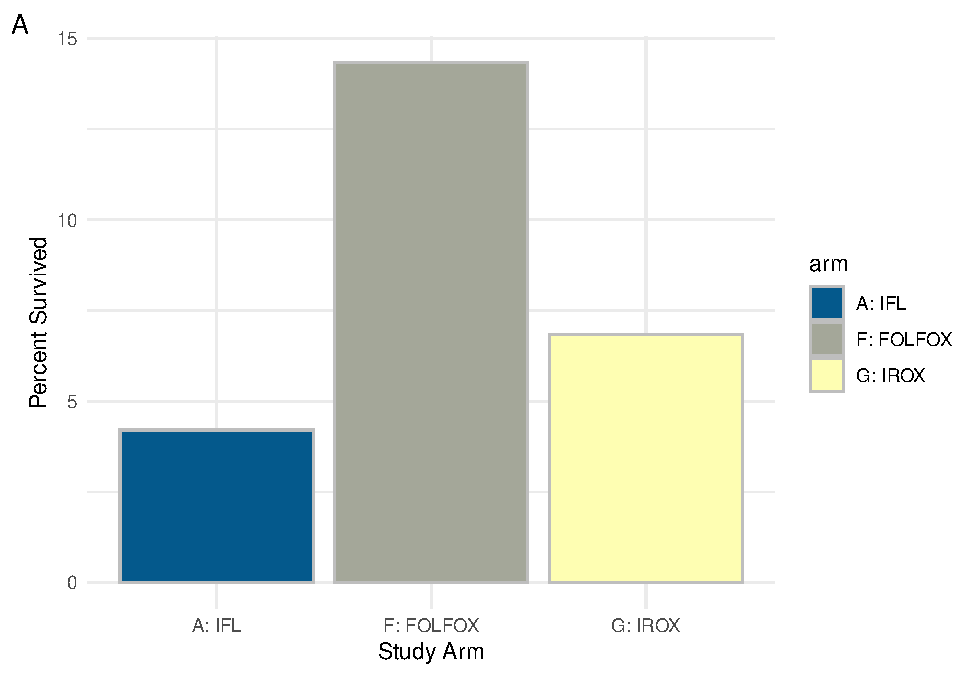
\includegraphics{04-paper_files/figure-latex/survival_barplot-1.pdf}

Then distribution plot of survival time (in days censored)

\begin{Shaded}
\begin{Highlighting}[]
\KeywordTok{ggplot}\NormalTok{(mockdata) }\OperatorTok{+}
\StringTok{  }\KeywordTok{aes}\NormalTok{(}\DataTypeTok{x=}\NormalTok{arm, }\DataTypeTok{y =}\NormalTok{ fu_time, }\DataTypeTok{fill=}\NormalTok{arm) }\OperatorTok{+}
\StringTok{  }\KeywordTok{geom_jitter}\NormalTok{(}\DataTypeTok{width =}\FloatTok{0.25}\NormalTok{, }\DataTypeTok{alpha=}\FloatTok{0.5}\NormalTok{) }\OperatorTok{+}
\StringTok{  }\KeywordTok{geom_violin}\NormalTok{(}\DataTypeTok{alpha =}\FloatTok{0.3}\NormalTok{) }\OperatorTok{+}
\StringTok{  }\KeywordTok{labs}\NormalTok{(}\DataTypeTok{y=} \StringTok{"Survival Time in }\CharTok{\textbackslash{}n}\StringTok{Days (Censored)"}\NormalTok{, }\DataTypeTok{x=} \StringTok{"Study Arm"}\NormalTok{, }\DataTypeTok{tag =} \StringTok{"B"}\NormalTok{) }\OperatorTok{+}
\StringTok{  }\KeywordTok{theme_minimal}\NormalTok{() }\OperatorTok{+}
\StringTok{  }\KeywordTok{scale_fill_scico_d}\NormalTok{(}\DataTypeTok{palette =} \StringTok{'nuuk'}\NormalTok{) ->}
\NormalTok{p2}

\NormalTok{p2}
\end{Highlighting}
\end{Shaded}

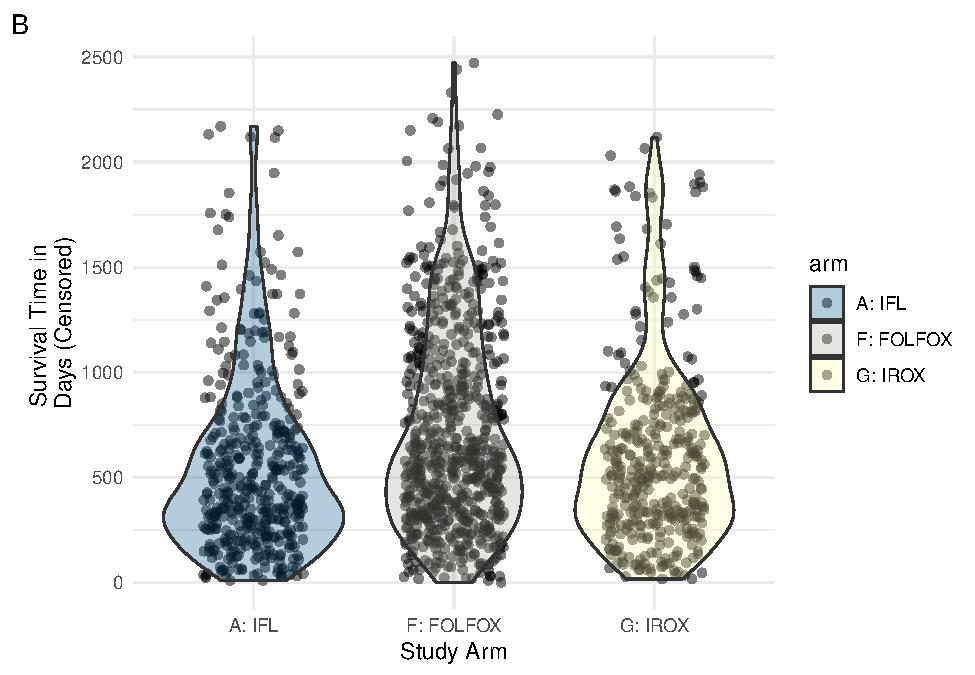
\includegraphics{04-paper_files/figure-latex/unnamed-chunk-8-1.pdf}

(for colors, maybe show \texttt{scale\_fill\_gray} + \texttt{scico})

\hypertarget{make-a-multi-panel-plot-here}{%
\section{Make a multi-panel plot here}\label{make-a-multi-panel-plot-here}}

\hypertarget{acknowledgments}{%
\subsection{Acknowledgments}\label{acknowledgments}}

This is a place to recognize people and institutions. It may also be a good place
to acknowledge and cite software that makes your work possible.

\hypertarget{author-contributions}{%
\subsection{Author Contributions}\label{author-contributions}}

We strongly encourage you to include an author contributions statement briefly
describing what each author did.



\end{document}
